\clearpage

\section{AliceQuantumTx}

\begin{tcolorbox}	
\begin{tabular}{p{2.75cm} p{0.2cm} p{10.5cm}} 	
\textbf{Header File}   &:& AliceQTx.h \\
\textbf{Source File}   &:& AliceQTx.cpp \\
\textbf{Version}       &:& 20190404
\end{tabular}
\end{tcolorbox}

\maketitle
This block is the quantum channel Alice's transmitter. This block accepts binary signals, which comprises the values for basis and bits to be used to encode single photons, as well as another binary value with modeSelection that selects the operation mode that Alice must operate.
\begin{itemize}
  \item inputSignal[0] $\rightarrow$ AliceQTxBasis (Binary)
  \item inputSignal[1] $\rightarrow$ AliceQTxBits (Binary)
  \item inputSignal[2] $\rightarrow$ ModeSelection (Binary)
\end{itemize}
It produces PhotonStreamXY signal which comprises the encoded single photons.
\begin{itemize}
  \item outputSignal[0] $\rightarrow$ AliceQTx\_Out (PhotonStreamXY)
\end{itemize}
It also accepts four input parameters listed below.

\subsection*{Input Parameters}

	\begin{itemize}
        \item string controlBasis - This string is the sequence of basis used to control qubits. Its default value is "0".

        \item string controlBits - This string is the sequence of bits used to control qubits. Its default value is "0".

		\item double numberOfPhotonsControl - Average number of photons contained in a control coherent pulse. Its default value is 80.
	
		\item double numberOfPhotonsData - Average number of photons contained in a data coherent pulse. Its default value is 1.

        \item int incrementControl - Increment to use in monitoring mode, i.e. for example if incrementControl is 100, Alice will transmit 1 control qubit in each 100 transmitted qubits. Its default value is 100;
	\end{itemize}

\subsection*{Methods}
\begin{itemize}
        \item void setControlBasisSequence(string bSeq) - This method allows to set the control basis sequence accepting a string value.

        \item void setControlBitsSequence(string bits) - This method allows to set the control bits sequence accepting a string value.

		\item void setNumberOfPhotonsData(double nData) - This method allows to set the average number of photons contained in data coherent pulses.
	
		\item void setNumberOfPhotonsControl(double nControl) - This method allows to set the average number of photons contained in control coherent pulses.

        \item void setIncrementControl(int inc) - This method allows to set the increment to use in monitoring mode.

\end{itemize}

\subsection*{Functional description}

\begin{figure}[h]
	\centering
	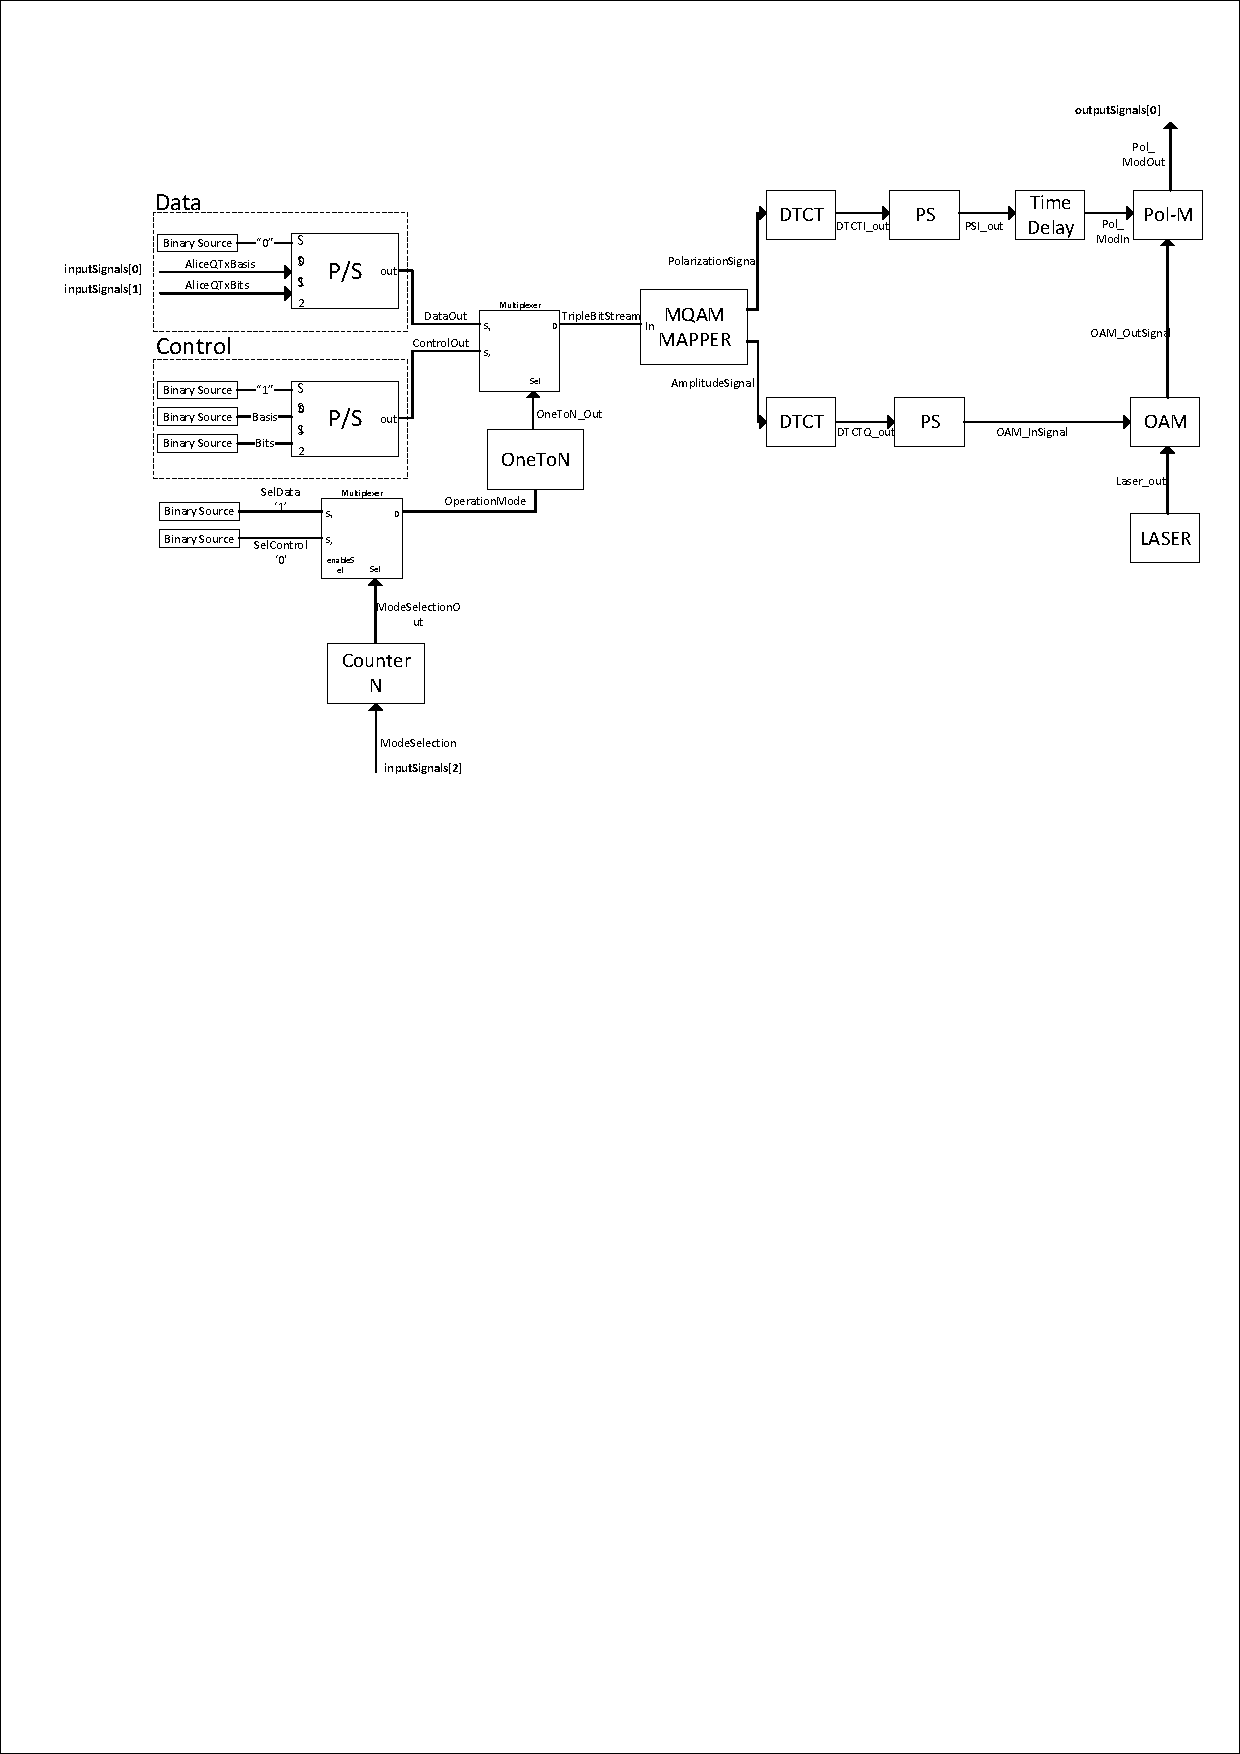
\includegraphics[clip, trim=0.5cm 15.0cm 0.5cm 0.1cm, width=1.0\textwidth]{./lib/AliceQuantumTx/figures/AliceQTx_diagram.pdf}
	\caption{Schematic of Alice Quantum Transmitter}\label{aliceQuantumTxDiagram}
\end{figure}

This block receives 3 input binary signals.

\begin{itemize}
        \item "ModeSelection" is a binary signal which gives to AliceQTx the information about operation mode, and so that she will know if she should send control or data qubits. If "ModeSelection" has the value "0" the monitoring mode is selected, and the output of this multiplexer will be a pre-defined sequence that should be "0" when data qubits are sent and "1" when control qubits are sent. This choice is made based on a sequence which should be deterministically made. Otherwise, if ModeSelection has the value "1", the actuation mode is selected and all qubits sent are control qubits.

        \item "AliceQTxBasis" is a binary signal which provides information about the basis to use to encode single-photons.

		\item "AliceQTxBits" is a binary signal which provides information about the bits to use to encode single-photons.
	
	\end{itemize}

"AliceQTxBasis" and "AliceQTxBits" will be responsible for data qubits encoding.

The operationMode signal will feed the other multiplex with an enable signal that should put on the output of the multiplexer, the input $s_2$ if this signal has the value "0" (control qubits), and the input $s_1$ if this signal has the value "1"(data qubits).

A triple bit stream binary signal outputs the multiplexer, where the sequence is $\{\textrm{Monitoring/Actuation}, \textrm{Basis}, \textrm{Bits}\}$, where the first bit is "0" if the actuation mode was selected, and "1" if the monitoring mode was selected. The MQAM Mapper block receives this bit stream and will be able to encode a constellation with 8 different symbols as shown in Figure \ref{AliceQTxconstellation}.

\begin{figure}[h]
	\centering
	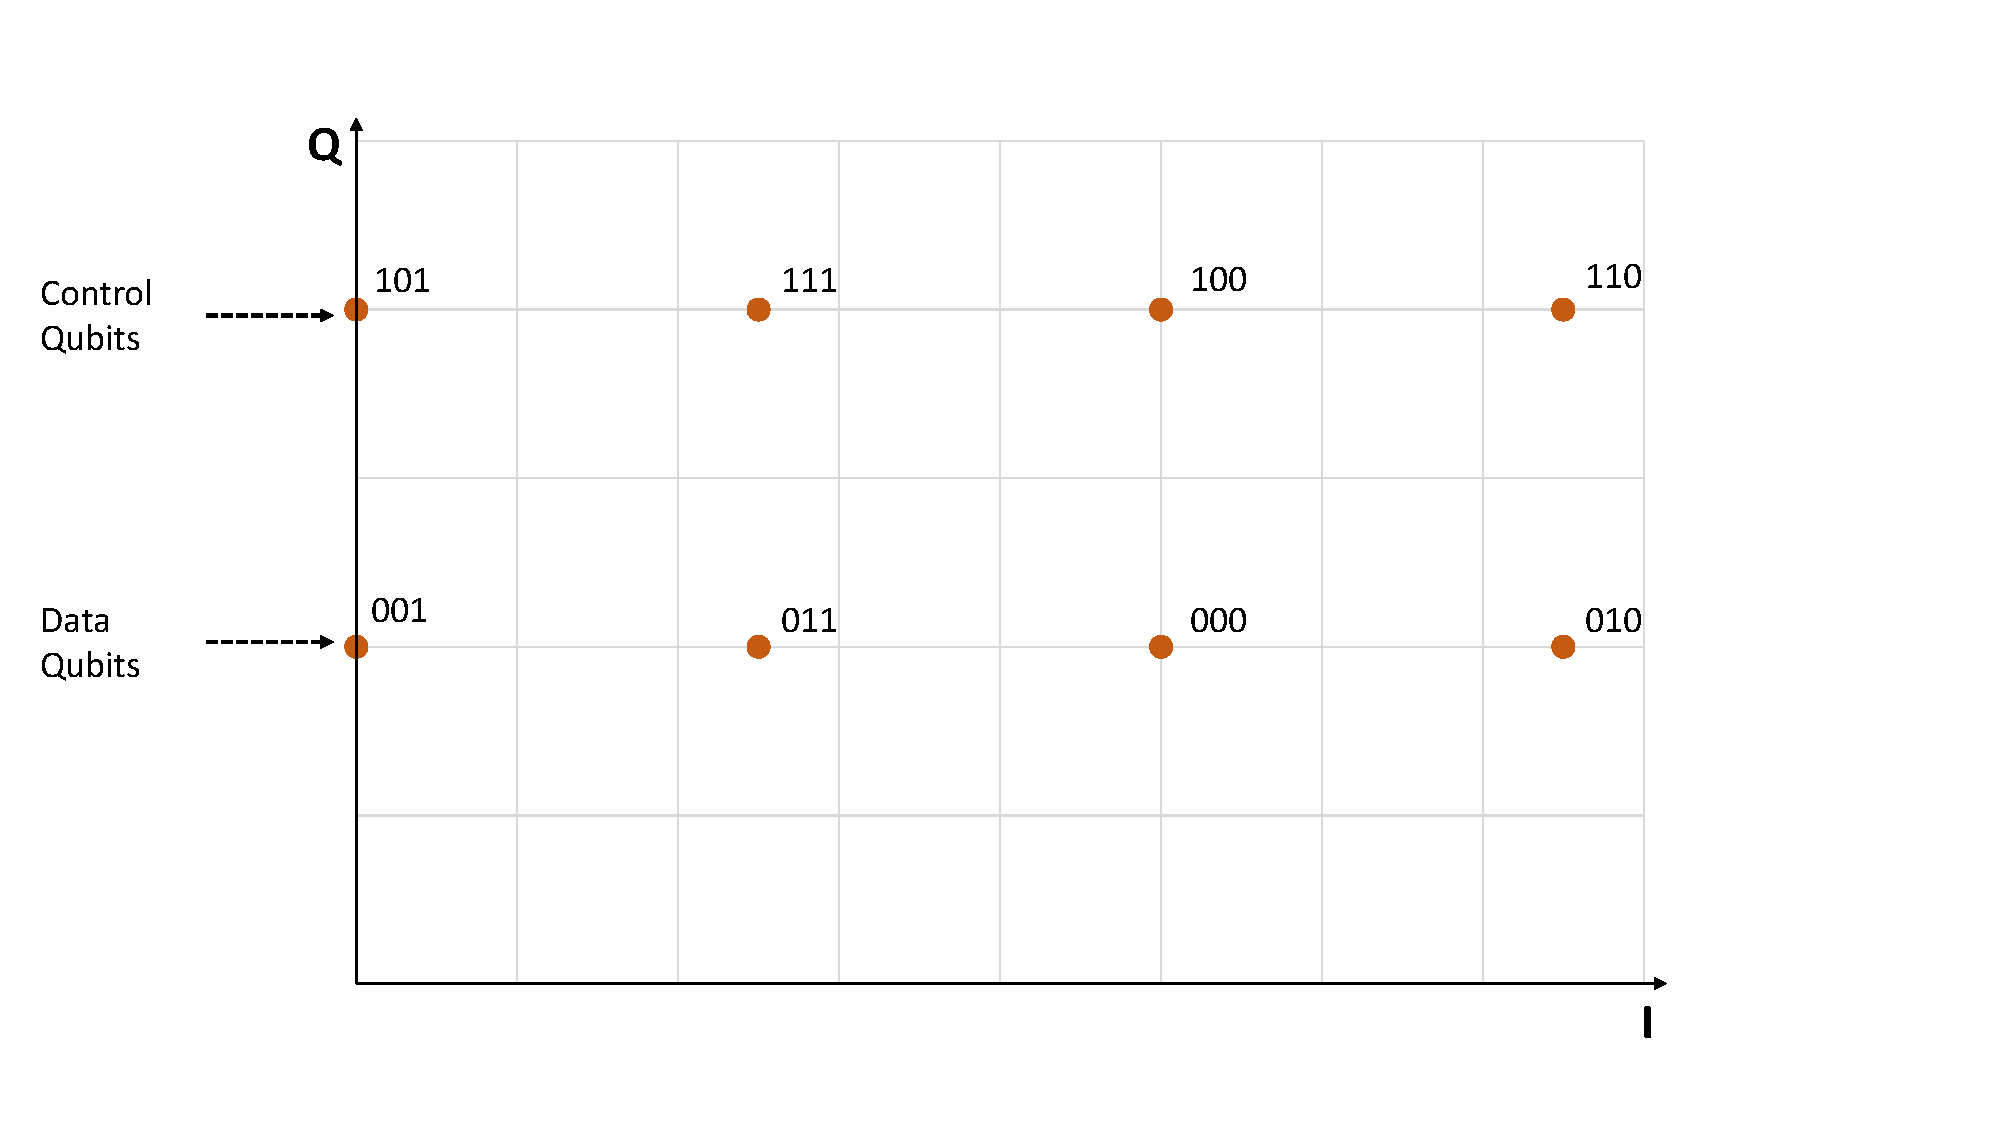
\includegraphics[clip, trim=0.5cm 0.5cm 0.5cm 0.5cm, width=1.0\textwidth]{./lib/AliceQuantumTx/figures/constellation.pdf}
	\caption{8 symbols constellation for Alice Quantum transmitter single photon codification.}\label{AliceQTxconstellation}
\end{figure}

The Quadrature component will provide an input signal for amplitude modulator, and it will modulate the signal according with two different amplitudes depending on the type of qubits to send, i.e. the control qubits will have higher amplitude than data qubits. The Intensity component will provide a signal with 4 different steps that will choose the polarization to encode the single photons. The amplitude modulator outputs a signal that enters in the polarization modulator and outputs with a certain polarization. At the output of Alice quantum transmitter there is a variable optical attenuator that will be responsible to reduce the number of photons per pulse until 0.1 for data qubits.

\subsection*{Input Signals}
\paragraph*{Number}: 3
\paragraph*{Type}: Binary.

\subsection*{Output Signals}
\paragraph*{Number}: 1
\paragraph*{Type}: PhotonStreamXY.

\subsection*{Examples}


\subsection*{Sugestions for future improvement}



